\documentclass[twoside]{book}

% Packages required by doxygen
\usepackage{fixltx2e}
\usepackage{calc}
\usepackage{doxygen}
\usepackage[export]{adjustbox} % also loads graphicx
\usepackage{graphicx}
\usepackage[utf8]{inputenc}
\usepackage{makeidx}
\usepackage{multicol}
\usepackage{multirow}
\PassOptionsToPackage{warn}{textcomp}
\usepackage{textcomp}
\usepackage[nointegrals]{wasysym}
\usepackage[table]{xcolor}

% NLS support packages
\usepackage[french]{babel}

% Font selection
\usepackage[T1]{fontenc}
\usepackage[scaled=.90]{helvet}
\usepackage{courier}
\usepackage{amssymb}
\usepackage{sectsty}
\renewcommand{\familydefault}{\sfdefault}
\allsectionsfont{%
  \fontseries{bc}\selectfont%
  \color{darkgray}%
}
\renewcommand{\DoxyLabelFont}{%
  \fontseries{bc}\selectfont%
  \color{darkgray}%
}
\newcommand{\+}{\discretionary{\mbox{\scriptsize$\hookleftarrow$}}{}{}}

% Page & text layout
\usepackage{geometry}
\geometry{%
  a4paper,%
  top=2.5cm,%
  bottom=2.5cm,%
  left=2.5cm,%
  right=2.5cm%
}
\tolerance=750
\hfuzz=15pt
\hbadness=750
\setlength{\emergencystretch}{15pt}
\setlength{\parindent}{0cm}
\setlength{\parskip}{3ex plus 2ex minus 2ex}
\makeatletter
\renewcommand{\paragraph}{%
  \@startsection{paragraph}{4}{0ex}{-1.0ex}{1.0ex}{%
    \normalfont\normalsize\bfseries\SS@parafont%
  }%
}
\renewcommand{\subparagraph}{%
  \@startsection{subparagraph}{5}{0ex}{-1.0ex}{1.0ex}{%
    \normalfont\normalsize\bfseries\SS@subparafont%
  }%
}
\makeatother

% Headers & footers
\usepackage{fancyhdr}
\pagestyle{fancyplain}
\fancyhead[LE]{\fancyplain{}{\bfseries\thepage}}
\fancyhead[CE]{\fancyplain{}{}}
\fancyhead[RE]{\fancyplain{}{\bfseries\leftmark}}
\fancyhead[LO]{\fancyplain{}{\bfseries\rightmark}}
\fancyhead[CO]{\fancyplain{}{}}
\fancyhead[RO]{\fancyplain{}{\bfseries\thepage}}
\fancyfoot[LE]{\fancyplain{}{}}
\fancyfoot[CE]{\fancyplain{}{}}
\fancyfoot[RE]{\fancyplain{}{\bfseries\scriptsize Généré par Doxygen }}
\fancyfoot[LO]{\fancyplain{}{\bfseries\scriptsize Généré par Doxygen }}
\fancyfoot[CO]{\fancyplain{}{}}
\fancyfoot[RO]{\fancyplain{}{}}
\renewcommand{\footrulewidth}{0.4pt}
\renewcommand{\chaptermark}[1]{%
  \markboth{#1}{}%
}
\renewcommand{\sectionmark}[1]{%
  \markright{\thesection\ #1}%
}

% Indices & bibliography
\usepackage{natbib}
\usepackage[titles]{tocloft}
\setcounter{tocdepth}{3}
\setcounter{secnumdepth}{5}
\makeindex

% Hyperlinks (required, but should be loaded last)
\usepackage{ifpdf}
\ifpdf
  \usepackage[pdftex,pagebackref=true]{hyperref}
\else
  \usepackage[ps2pdf,pagebackref=true]{hyperref}
\fi
\hypersetup{%
  colorlinks=true,%
  linkcolor=blue,%
  citecolor=blue,%
  unicode%
}

% Custom commands
\newcommand{\clearemptydoublepage}{%
  \newpage{\pagestyle{empty}\cleardoublepage}%
}

\usepackage{caption}
\captionsetup{labelsep=space,justification=centering,font={bf},singlelinecheck=off,skip=4pt,position=top}

%===== C O N T E N T S =====

\begin{document}

% Titlepage & ToC
\hypersetup{pageanchor=false,
             bookmarksnumbered=true,
             pdfencoding=unicode
            }
\pagenumbering{alph}
\begin{titlepage}
\vspace*{7cm}
\begin{center}%
{\Large T\+P4 -\/ Simulation d\textquotesingle{}une population de lapins }\\
\vspace*{1cm}
{\large Généré par Doxygen 1.8.13}\\
\end{center}
\end{titlepage}
\clearemptydoublepage
\pagenumbering{roman}
\tableofcontents
\clearemptydoublepage
\pagenumbering{arabic}
\hypersetup{pageanchor=true}

%--- Begin generated contents ---
\chapter{Index hiérarchique}
\section{Hiérarchie des classes}
Cette liste d\textquotesingle{}héritage est classée approximativement par ordre alphabétique \+:\begin{DoxyCompactList}
\item \contentsline{section}{Population}{\pageref{classPopulation}}{}
\item \contentsline{section}{Rabbit}{\pageref{classRabbit}}{}
\begin{DoxyCompactList}
\item \contentsline{section}{Female\+Rabbit}{\pageref{classFemaleRabbit}}{}
\end{DoxyCompactList}
\end{DoxyCompactList}

\chapter{Index des classes}
\section{Structures de données}
Liste des structures de données avec une brève description \+:\begin{DoxyCompactList}
\item\contentsline{section}{\hyperlink{classFemaleRabbit}{Female\+Rabbit} \\*Classe représentant un lapin femelle }{\pageref{classFemaleRabbit}}{}
\item\contentsline{section}{\hyperlink{classPopulation}{Population} \\*Représente une population de lapins }{\pageref{classPopulation}}{}
\item\contentsline{section}{\hyperlink{classRabbit}{Rabbit} \\*Classe représentant un lapin (mâle ou femelle) }{\pageref{classRabbit}}{}
\end{DoxyCompactList}

\chapter{Index des fichiers}
\section{Liste des fichiers}
Liste de tous les fichiers avec une brève description \+:\begin{DoxyCompactList}
\item\contentsline{section}{\hyperlink{main_8c}{main.\+c} \\*Implémentations et tests des fonctions créees pour le TP n°3 de Simulation }{\pageref{main_8c}}{}
\end{DoxyCompactList}

\chapter{Documentation des classes}
\hypertarget{classRabbit}{}\section{Référence de la classe Rabbit}
\label{classRabbit}\index{Rabbit@{Rabbit}}


Classe représentant un lapin (mâle ou femelle)  




{\ttfamily \#include $<$Rabbit.\+hpp$>$}



Graphe d\textquotesingle{}héritage de Rabbit\+:
\nopagebreak
\begin{figure}[H]
\begin{center}
\leavevmode
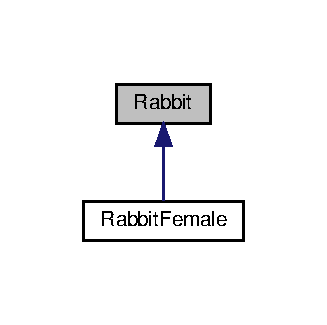
\includegraphics[width=157pt]{classRabbit__inherit__graph}
\end{center}
\end{figure}
\subsection*{Fonctions membres publiques}
\begin{DoxyCompactItemize}
\item 
\hyperlink{classRabbit_ae2093988d2ba8f561213a9767e8a31dd}{Rabbit} ()
\begin{DoxyCompactList}\small\item\em Construit un nouvel objet \char`\"{}\+Rabbit\char`\"{}. \end{DoxyCompactList}\item 
virtual \hyperlink{classRabbit_ac57586ffc31fffa6392638afbbd32774}{$\sim$\+Rabbit} ()
\begin{DoxyCompactList}\small\item\em Détruit l\textquotesingle{}objet \char`\"{}\+Rabbit\char`\"{}. \end{DoxyCompactList}\item 
virtual void \hyperlink{classRabbit_a404af8877c99ddc98108d88c8e466013}{grow} ()
\begin{DoxyCompactList}\small\item\em Méthode qui fait veillir l\textquotesingle{}instance d\textquotesingle{}un lapin de 1 mois. \end{DoxyCompactList}\item 
bool \hyperlink{classRabbit_a8087ee3ab0acaa6108e6982933b0f79a}{has\+Majority} () const
\begin{DoxyCompactList}\small\item\em Méthode pour savoir si le lapin est jeune ou adulte. \end{DoxyCompactList}\item 
bool \hyperlink{classRabbit_a82cf75bd520aaa775fadbf103fc12499}{has\+To\+Die} () const
\begin{DoxyCompactList}\small\item\em Méthode pour savoir si le lapin doit mourir ce mois. \end{DoxyCompactList}\item 
unsigned int \hyperlink{classRabbit_ab34450717cf7b3f9eb22747527c34922}{get\+Age} () const
\begin{DoxyCompactList}\small\item\em Getter pour l\textquotesingle{}age. \end{DoxyCompactList}\item 
virtual bool \hyperlink{classRabbit_a913437a589519afdb9249825bd6f03bd}{is\+Male} () const
\begin{DoxyCompactList}\small\item\em Méthode permettant de savoir si l\textquotesingle{}instance est celle d\textquotesingle{}un lapin mâle ou femelle. \end{DoxyCompactList}\end{DoxyCompactItemize}
\subsection*{Attributs publics statiques}
\begin{DoxyCompactItemize}
\item 
static constexpr double \hyperlink{classRabbit_ac6dc736f2b0395fa8692461a457a5297}{survival\+\_\+proba\+\_\+young} = 0.\+2
\begin{DoxyCompactList}\small\item\em probabilité de survivre à la jeunesse (les 5 à 8 premiers mois) \end{DoxyCompactList}\item 
static constexpr double \hyperlink{classRabbit_a8b8affe7fcdc56e08da384d8d82ec556}{survival\+\_\+proba\+\_\+adult} = 0.\+5
\begin{DoxyCompactList}\small\item\em probabilité de survivre pour un lapin adulte (11 ans moins les mois de jeunesse) \end{DoxyCompactList}\end{DoxyCompactItemize}
\subsection*{Attributs protégés}
\begin{DoxyCompactItemize}
\item 
unsigned int \hyperlink{classRabbit_a396c4c8693ea4f827f12afd6d1320ec0}{\+\_\+age}
\begin{DoxyCompactList}\small\item\em L\textquotesingle{}age du lapin en mois. \end{DoxyCompactList}\item 
unsigned int \hyperlink{classRabbit_a7cf441478e82d384166605c69f99f39e}{\+\_\+majority}
\begin{DoxyCompactList}\small\item\em Nombre de mois avant que le lapin n\textquotesingle{}atteigne la majorité et passe à l\textquotesingle{}age adulte et puisse enfanter (si c\textquotesingle{}est une femelle) \end{DoxyCompactList}\item 
double \hyperlink{classRabbit_a622452eedf7ef0addf1e2ce3d8ef34dc}{\+\_\+proba\+\_\+to\+\_\+die\+\_\+young}
\begin{DoxyCompactList}\small\item\em Probabilité de mourir (par mois) avant de devenir adulte, calculée avec la probabilité de survivre et le nombre de mois de jeunesse. \end{DoxyCompactList}\item 
double \hyperlink{classRabbit_a600d8595c407b95965497f7308d72ab1}{\+\_\+proba\+\_\+to\+\_\+die\+\_\+adult}
\begin{DoxyCompactList}\small\item\em Probabilité de mourir (par mois) en étant adulte, calculée avec la probabilité de survivre et le nombre de mois de jeunesse. \end{DoxyCompactList}\end{DoxyCompactItemize}


\subsection{Description détaillée}
Classe représentant un lapin (mâle ou femelle) 

Si l\textquotesingle{}objet est créé en tant que \hyperlink{classRabbit}{Rabbit}, c\textquotesingle{}est qu\textquotesingle{}il représente un lapin mâle, sinon la classe utilisée sera \hyperlink{classFemaleRabbit}{Female\+Rabbit}. Cependant la classe \hyperlink{classRabbit}{Rabbit} synthétise les deux genres. Il n\textquotesingle{}y a juste pas de classe Male\+Rabbit puisque celle-\/ci n\textquotesingle{}implémenterait rien de plus que la classe \hyperlink{classRabbit}{Rabbit}. 

Définition à la ligne 23 du fichier Rabbit.\+hpp.



\subsection{Documentation des constructeurs et destructeur}
\mbox{\Hypertarget{classRabbit_ae2093988d2ba8f561213a9767e8a31dd}\label{classRabbit_ae2093988d2ba8f561213a9767e8a31dd}} 
\index{Rabbit@{Rabbit}!Rabbit@{Rabbit}}
\index{Rabbit@{Rabbit}!Rabbit@{Rabbit}}
\subsubsection{\texorpdfstring{Rabbit()}{Rabbit()}}
{\footnotesize\ttfamily Rabbit\+::\+Rabbit (\begin{DoxyParamCaption}{ }\end{DoxyParamCaption})}



Construit un nouvel objet \char`\"{}\+Rabbit\char`\"{}. 

Définit l\textquotesingle{}age de la majorité, la probabilité de mourir jeune et la probabilité de mourir en étant adulte 

Définition à la ligne 18 du fichier Rabbit.\+cpp.

Voici le graphe des appelants de cette fonction \+:
\nopagebreak
\begin{figure}[H]
\begin{center}
\leavevmode
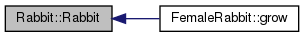
\includegraphics[width=300pt]{classRabbit_ae2093988d2ba8f561213a9767e8a31dd_icgraph}
\end{center}
\end{figure}
\mbox{\Hypertarget{classRabbit_ac57586ffc31fffa6392638afbbd32774}\label{classRabbit_ac57586ffc31fffa6392638afbbd32774}} 
\index{Rabbit@{Rabbit}!````~Rabbit@{$\sim$\+Rabbit}}
\index{````~Rabbit@{$\sim$\+Rabbit}!Rabbit@{Rabbit}}
\subsubsection{\texorpdfstring{$\sim$\+Rabbit()}{~Rabbit()}}
{\footnotesize\ttfamily Rabbit\+::$\sim$\+Rabbit (\begin{DoxyParamCaption}{ }\end{DoxyParamCaption})\hspace{0.3cm}{\ttfamily [virtual]}}



Détruit l\textquotesingle{}objet \char`\"{}\+Rabbit\char`\"{}. 



Définition à la ligne 29 du fichier Rabbit.\+cpp.



\subsection{Documentation des fonctions membres}
\mbox{\Hypertarget{classRabbit_ab34450717cf7b3f9eb22747527c34922}\label{classRabbit_ab34450717cf7b3f9eb22747527c34922}} 
\index{Rabbit@{Rabbit}!get\+Age@{get\+Age}}
\index{get\+Age@{get\+Age}!Rabbit@{Rabbit}}
\subsubsection{\texorpdfstring{get\+Age()}{getAge()}}
{\footnotesize\ttfamily unsigned int Rabbit\+::get\+Age (\begin{DoxyParamCaption}{ }\end{DoxyParamCaption}) const}



Getter pour l\textquotesingle{}age. 

\begin{DoxyReturn}{Renvoie}
unsigned int l\textquotesingle{}age du lapin 
\end{DoxyReturn}


Définition à la ligne 68 du fichier Rabbit.\+cpp.

\mbox{\Hypertarget{classRabbit_a404af8877c99ddc98108d88c8e466013}\label{classRabbit_a404af8877c99ddc98108d88c8e466013}} 
\index{Rabbit@{Rabbit}!grow@{grow}}
\index{grow@{grow}!Rabbit@{Rabbit}}
\subsubsection{\texorpdfstring{grow()}{grow()}}
{\footnotesize\ttfamily void Rabbit\+::grow (\begin{DoxyParamCaption}{ }\end{DoxyParamCaption})\hspace{0.3cm}{\ttfamily [virtual]}}



Méthode qui fait veillir l\textquotesingle{}instance d\textquotesingle{}un lapin de 1 mois. 



Réimplémentée dans \hyperlink{classFemaleRabbit_ad938ea7eca97c53e89d11392b6856ebd}{Female\+Rabbit}.



Définition à la ligne 36 du fichier Rabbit.\+cpp.

Voici le graphe des appelants de cette fonction \+:
\nopagebreak
\begin{figure}[H]
\begin{center}
\leavevmode
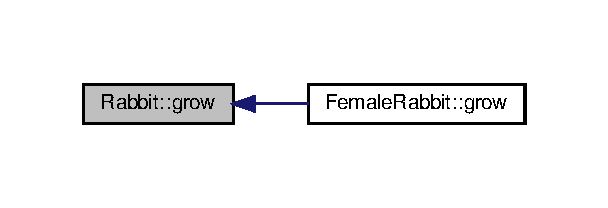
\includegraphics[width=292pt]{classRabbit_a404af8877c99ddc98108d88c8e466013_icgraph}
\end{center}
\end{figure}
\mbox{\Hypertarget{classRabbit_a8087ee3ab0acaa6108e6982933b0f79a}\label{classRabbit_a8087ee3ab0acaa6108e6982933b0f79a}} 
\index{Rabbit@{Rabbit}!has\+Majority@{has\+Majority}}
\index{has\+Majority@{has\+Majority}!Rabbit@{Rabbit}}
\subsubsection{\texorpdfstring{has\+Majority()}{hasMajority()}}
{\footnotesize\ttfamily bool Rabbit\+::has\+Majority (\begin{DoxyParamCaption}{ }\end{DoxyParamCaption}) const}



Méthode pour savoir si le lapin est jeune ou adulte. 

\begin{DoxyReturn}{Renvoie}
true si le lapin est adulte 

false si le lapin est jeune 
\end{DoxyReturn}


Définition à la ligne 47 du fichier Rabbit.\+cpp.

Voici le graphe des appelants de cette fonction \+:
\nopagebreak
\begin{figure}[H]
\begin{center}
\leavevmode
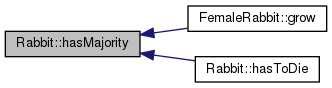
\includegraphics[width=321pt]{classRabbit_a8087ee3ab0acaa6108e6982933b0f79a_icgraph}
\end{center}
\end{figure}
\mbox{\Hypertarget{classRabbit_a82cf75bd520aaa775fadbf103fc12499}\label{classRabbit_a82cf75bd520aaa775fadbf103fc12499}} 
\index{Rabbit@{Rabbit}!has\+To\+Die@{has\+To\+Die}}
\index{has\+To\+Die@{has\+To\+Die}!Rabbit@{Rabbit}}
\subsubsection{\texorpdfstring{has\+To\+Die()}{hasToDie()}}
{\footnotesize\ttfamily bool Rabbit\+::has\+To\+Die (\begin{DoxyParamCaption}{ }\end{DoxyParamCaption}) const}



Méthode pour savoir si le lapin doit mourir ce mois. 

\begin{DoxyReturn}{Renvoie}
true si il doit mourir 

false si il survit 
\end{DoxyReturn}


Définition à la ligne 58 du fichier Rabbit.\+cpp.

Voici le graphe d\textquotesingle{}appel pour cette fonction \+:
\nopagebreak
\begin{figure}[H]
\begin{center}
\leavevmode
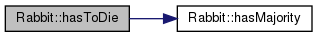
\includegraphics[width=310pt]{classRabbit_a82cf75bd520aaa775fadbf103fc12499_cgraph}
\end{center}
\end{figure}
\mbox{\Hypertarget{classRabbit_a913437a589519afdb9249825bd6f03bd}\label{classRabbit_a913437a589519afdb9249825bd6f03bd}} 
\index{Rabbit@{Rabbit}!is\+Male@{is\+Male}}
\index{is\+Male@{is\+Male}!Rabbit@{Rabbit}}
\subsubsection{\texorpdfstring{is\+Male()}{isMale()}}
{\footnotesize\ttfamily bool Rabbit\+::is\+Male (\begin{DoxyParamCaption}{ }\end{DoxyParamCaption}) const\hspace{0.3cm}{\ttfamily [virtual]}}



Méthode permettant de savoir si l\textquotesingle{}instance est celle d\textquotesingle{}un lapin mâle ou femelle. 



Réimplémentée dans \hyperlink{classFemaleRabbit_a60250dbc3758c7d31537f13b4879fe33}{Female\+Rabbit}.



Définition à la ligne 76 du fichier Rabbit.\+cpp.



\subsection{Documentation des champs}
\mbox{\Hypertarget{classRabbit_a396c4c8693ea4f827f12afd6d1320ec0}\label{classRabbit_a396c4c8693ea4f827f12afd6d1320ec0}} 
\index{Rabbit@{Rabbit}!\+\_\+age@{\+\_\+age}}
\index{\+\_\+age@{\+\_\+age}!Rabbit@{Rabbit}}
\subsubsection{\texorpdfstring{\+\_\+age}{\_age}}
{\footnotesize\ttfamily unsigned int Rabbit\+::\+\_\+age\hspace{0.3cm}{\ttfamily [protected]}}



L\textquotesingle{}age du lapin en mois. 



Définition à la ligne 39 du fichier Rabbit.\+hpp.

\mbox{\Hypertarget{classRabbit_a7cf441478e82d384166605c69f99f39e}\label{classRabbit_a7cf441478e82d384166605c69f99f39e}} 
\index{Rabbit@{Rabbit}!\+\_\+majority@{\+\_\+majority}}
\index{\+\_\+majority@{\+\_\+majority}!Rabbit@{Rabbit}}
\subsubsection{\texorpdfstring{\+\_\+majority}{\_majority}}
{\footnotesize\ttfamily unsigned int Rabbit\+::\+\_\+majority\hspace{0.3cm}{\ttfamily [protected]}}



Nombre de mois avant que le lapin n\textquotesingle{}atteigne la majorité et passe à l\textquotesingle{}age adulte et puisse enfanter (si c\textquotesingle{}est une femelle) 



Définition à la ligne 40 du fichier Rabbit.\+hpp.

\mbox{\Hypertarget{classRabbit_a600d8595c407b95965497f7308d72ab1}\label{classRabbit_a600d8595c407b95965497f7308d72ab1}} 
\index{Rabbit@{Rabbit}!\+\_\+proba\+\_\+to\+\_\+die\+\_\+adult@{\+\_\+proba\+\_\+to\+\_\+die\+\_\+adult}}
\index{\+\_\+proba\+\_\+to\+\_\+die\+\_\+adult@{\+\_\+proba\+\_\+to\+\_\+die\+\_\+adult}!Rabbit@{Rabbit}}
\subsubsection{\texorpdfstring{\+\_\+proba\+\_\+to\+\_\+die\+\_\+adult}{\_proba\_to\_die\_adult}}
{\footnotesize\ttfamily double Rabbit\+::\+\_\+proba\+\_\+to\+\_\+die\+\_\+adult\hspace{0.3cm}{\ttfamily [protected]}}



Probabilité de mourir (par mois) en étant adulte, calculée avec la probabilité de survivre et le nombre de mois de jeunesse. 



Définition à la ligne 42 du fichier Rabbit.\+hpp.

\mbox{\Hypertarget{classRabbit_a622452eedf7ef0addf1e2ce3d8ef34dc}\label{classRabbit_a622452eedf7ef0addf1e2ce3d8ef34dc}} 
\index{Rabbit@{Rabbit}!\+\_\+proba\+\_\+to\+\_\+die\+\_\+young@{\+\_\+proba\+\_\+to\+\_\+die\+\_\+young}}
\index{\+\_\+proba\+\_\+to\+\_\+die\+\_\+young@{\+\_\+proba\+\_\+to\+\_\+die\+\_\+young}!Rabbit@{Rabbit}}
\subsubsection{\texorpdfstring{\+\_\+proba\+\_\+to\+\_\+die\+\_\+young}{\_proba\_to\_die\_young}}
{\footnotesize\ttfamily double Rabbit\+::\+\_\+proba\+\_\+to\+\_\+die\+\_\+young\hspace{0.3cm}{\ttfamily [protected]}}



Probabilité de mourir (par mois) avant de devenir adulte, calculée avec la probabilité de survivre et le nombre de mois de jeunesse. 



Définition à la ligne 41 du fichier Rabbit.\+hpp.

\mbox{\Hypertarget{classRabbit_a8b8affe7fcdc56e08da384d8d82ec556}\label{classRabbit_a8b8affe7fcdc56e08da384d8d82ec556}} 
\index{Rabbit@{Rabbit}!survival\+\_\+proba\+\_\+adult@{survival\+\_\+proba\+\_\+adult}}
\index{survival\+\_\+proba\+\_\+adult@{survival\+\_\+proba\+\_\+adult}!Rabbit@{Rabbit}}
\subsubsection{\texorpdfstring{survival\+\_\+proba\+\_\+adult}{survival\_proba\_adult}}
{\footnotesize\ttfamily constexpr double Rabbit\+::survival\+\_\+proba\+\_\+adult = 0.\+5\hspace{0.3cm}{\ttfamily [static]}}



probabilité de survivre pour un lapin adulte (11 ans moins les mois de jeunesse) 



Définition à la ligne 36 du fichier Rabbit.\+hpp.

\mbox{\Hypertarget{classRabbit_ac6dc736f2b0395fa8692461a457a5297}\label{classRabbit_ac6dc736f2b0395fa8692461a457a5297}} 
\index{Rabbit@{Rabbit}!survival\+\_\+proba\+\_\+young@{survival\+\_\+proba\+\_\+young}}
\index{survival\+\_\+proba\+\_\+young@{survival\+\_\+proba\+\_\+young}!Rabbit@{Rabbit}}
\subsubsection{\texorpdfstring{survival\+\_\+proba\+\_\+young}{survival\_proba\_young}}
{\footnotesize\ttfamily constexpr double Rabbit\+::survival\+\_\+proba\+\_\+young = 0.\+2\hspace{0.3cm}{\ttfamily [static]}}



probabilité de survivre à la jeunesse (les 5 à 8 premiers mois) 



Définition à la ligne 35 du fichier Rabbit.\+hpp.



La documentation de cette classe a été générée à partir des fichiers suivants \+:\begin{DoxyCompactItemize}
\item 
\hyperlink{Rabbit_8hpp}{Rabbit.\+hpp}\item 
\hyperlink{Rabbit_8cpp}{Rabbit.\+cpp}\end{DoxyCompactItemize}

\hypertarget{classRabbitFemale}{}\section{Référence de la classe Rabbit\+Female}
\label{classRabbitFemale}\index{Rabbit\+Female@{Rabbit\+Female}}


Graphe d\textquotesingle{}héritage de Rabbit\+Female\+:\nopagebreak
\begin{figure}[H]
\begin{center}
\leavevmode
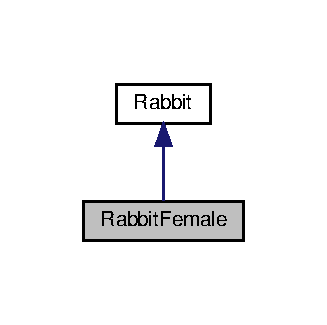
\includegraphics[width=157pt]{classRabbitFemale__inherit__graph}
\end{center}
\end{figure}


Graphe de collaboration de Rabbit\+Female\+:\nopagebreak
\begin{figure}[H]
\begin{center}
\leavevmode
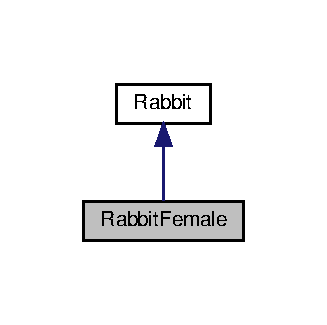
\includegraphics[width=157pt]{classRabbitFemale__coll__graph}
\end{center}
\end{figure}
\subsection*{Fonctions membres publiques}
\begin{DoxyCompactItemize}
\item 
\hyperlink{classRabbitFemale_afc3b2704f27fcf00365f4c3e8bd833bd}{Rabbit\+Female} (unsigned int week\+\_\+offset=0)
\begin{DoxyCompactList}\small\item\em Construction d\textquotesingle{}un nouveau \hyperlink{classRabbit}{Rabbit} Female\+:\+: \hyperlink{classRabbit}{Rabbit} Female. \end{DoxyCompactList}\item 
\hyperlink{classRabbitFemale_a647e3ccc4f2def58440a8faf2855d579}{$\sim$\+Rabbit\+Female} ()
\begin{DoxyCompactList}\small\item\em Destruction de l\textquotesingle{}objet \hyperlink{classRabbit}{Rabbit} Female\+:\+: \hyperlink{classRabbit}{Rabbit} Female. \end{DoxyCompactList}\item 
void \hyperlink{classRabbitFemale_adc6ed8ce0605e19fcbc2c21ac43db8ee}{give\+\_\+birth} (unsigned int week, std\+::list$<$ \hyperlink{classRabbit}{Rabbit} $\ast$$>$ \&males, std\+::list$<$ \hyperlink{classRabbitFemale}{Rabbit\+Female} $\ast$$>$ \&females)
\begin{DoxyCompactList}\small\item\em Donne naissance à une portée si nécessaire. \end{DoxyCompactList}\end{DoxyCompactItemize}
\subsection*{Membres hérités additionnels}


\subsection{Documentation des constructeurs et destructeur}
\mbox{\Hypertarget{classRabbitFemale_afc3b2704f27fcf00365f4c3e8bd833bd}\label{classRabbitFemale_afc3b2704f27fcf00365f4c3e8bd833bd}} 
\index{Rabbit\+Female@{Rabbit\+Female}!Rabbit\+Female@{Rabbit\+Female}}
\index{Rabbit\+Female@{Rabbit\+Female}!Rabbit\+Female@{Rabbit\+Female}}
\subsubsection{\texorpdfstring{Rabbit\+Female()}{RabbitFemale()}}
{\footnotesize\ttfamily Rabbit\+Female\+::\+Rabbit\+Female (\begin{DoxyParamCaption}\item[{unsigned int}]{week\+\_\+offset = {\ttfamily 0} }\end{DoxyParamCaption})}



Construction d\textquotesingle{}un nouveau \hyperlink{classRabbit}{Rabbit} Female\+:\+: \hyperlink{classRabbit}{Rabbit} Female. 


\begin{DoxyParams}{Paramètres}
{\em week\+\_\+offset} & décalage entre l\textquotesingle{}échelle temporelle de la simulation et celle du lapin. \\
\hline
\end{DoxyParams}
\mbox{\Hypertarget{classRabbitFemale_a647e3ccc4f2def58440a8faf2855d579}\label{classRabbitFemale_a647e3ccc4f2def58440a8faf2855d579}} 
\index{Rabbit\+Female@{Rabbit\+Female}!````~Rabbit\+Female@{$\sim$\+Rabbit\+Female}}
\index{````~Rabbit\+Female@{$\sim$\+Rabbit\+Female}!Rabbit\+Female@{Rabbit\+Female}}
\subsubsection{\texorpdfstring{$\sim$\+Rabbit\+Female()}{~RabbitFemale()}}
{\footnotesize\ttfamily Rabbit\+Female\+::$\sim$\+Rabbit\+Female (\begin{DoxyParamCaption}{ }\end{DoxyParamCaption})}



Destruction de l\textquotesingle{}objet \hyperlink{classRabbit}{Rabbit} Female\+:\+: \hyperlink{classRabbit}{Rabbit} Female. 

Libération de la mémoire allouée aux portées 

\subsection{Documentation des fonctions membres}
\mbox{\Hypertarget{classRabbitFemale_adc6ed8ce0605e19fcbc2c21ac43db8ee}\label{classRabbitFemale_adc6ed8ce0605e19fcbc2c21ac43db8ee}} 
\index{Rabbit\+Female@{Rabbit\+Female}!give\+\_\+birth@{give\+\_\+birth}}
\index{give\+\_\+birth@{give\+\_\+birth}!Rabbit\+Female@{Rabbit\+Female}}
\subsubsection{\texorpdfstring{give\+\_\+birth()}{give\_birth()}}
{\footnotesize\ttfamily void Rabbit\+Female\+::give\+\_\+birth (\begin{DoxyParamCaption}\item[{unsigned int}]{week,  }\item[{std\+::list$<$ \hyperlink{classRabbit}{Rabbit} $\ast$$>$ \&}]{males,  }\item[{std\+::list$<$ \hyperlink{classRabbitFemale}{Rabbit\+Female} $\ast$$>$ \&}]{females }\end{DoxyParamCaption})}



Donne naissance à une portée si nécessaire. 


\begin{DoxyParams}{Paramètres}
{\em week} & date actuelle de la simulation \\
\hline
{\em males} & liste des mâles appartenant à la simulation \\
\hline
{\em females} & liste des femelles appartenant à la simulation \\
\hline
\end{DoxyParams}


La documentation de cette classe a été générée à partir des fichiers suivants \+:\begin{DoxyCompactItemize}
\item 
\hyperlink{RabbitFemale_8hpp}{Rabbit\+Female.\+hpp}\item 
\hyperlink{RabbitFemale_8cpp}{Rabbit\+Female.\+cpp}\end{DoxyCompactItemize}

\hypertarget{classRabbitSimulation}{}\section{Référence de la classe Rabbit\+Simulation}
\label{classRabbitSimulation}\index{Rabbit\+Simulation@{Rabbit\+Simulation}}
\subsection*{Fonctions membres publiques}
\begin{DoxyCompactItemize}
\item 
\mbox{\Hypertarget{classRabbitSimulation_a7cff4ba08c71c15ee2eb109128a48c5c}\label{classRabbitSimulation_a7cff4ba08c71c15ee2eb109128a48c5c}} 
{\bfseries Rabbit\+Simulation} (unsigned int nb\+\_\+males\+\_\+init=2, unsigned int nb\+\_\+females\+\_\+init=2)
\item 
\mbox{\Hypertarget{classRabbitSimulation_a8c033edc85bb3b72a4704e48ba699e20}\label{classRabbitSimulation_a8c033edc85bb3b72a4704e48ba699e20}} 
void {\bfseries run} (unsigned int week)
\end{DoxyCompactItemize}


La documentation de cette classe a été générée à partir des fichiers suivants \+:\begin{DoxyCompactItemize}
\item 
\hyperlink{RabbitSimulation_8hpp}{Rabbit\+Simulation.\+hpp}\item 
Rabbit\+Simulation.\+cpp\end{DoxyCompactItemize}

\chapter{Documentation des fichiers}
\hypertarget{Rabbit_8cpp}{}\section{Référence du fichier Rabbit.\+cpp}
\label{Rabbit_8cpp}\index{Rabbit.\+cpp@{Rabbit.\+cpp}}


Fichier d\textquotesingle{}implémentation de la classe \hyperlink{classRabbit}{Rabbit}.  


{\ttfamily \#include \char`\"{}Rabbit.\+hpp\char`\"{}}\newline
Graphe des dépendances par inclusion de Rabbit.\+cpp\+:
\nopagebreak
\begin{figure}[H]
\begin{center}
\leavevmode
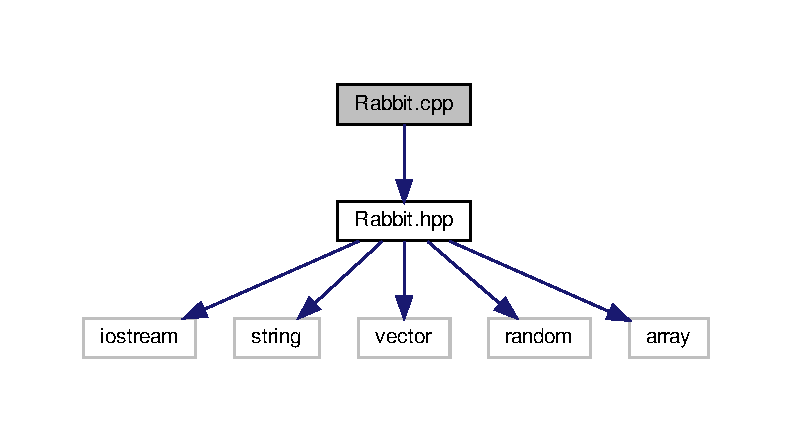
\includegraphics[width=350pt]{Rabbit_8cpp__incl}
\end{center}
\end{figure}


\subsection{Description détaillée}
Fichier d\textquotesingle{}implémentation de la classe \hyperlink{classRabbit}{Rabbit}. 

\begin{DoxyAuthor}{Auteur}
Mathieu Arquilliere (\href{mailto:mathieu.arquilliere@etu.uca.fr}{\tt mathieu.\+arquilliere@etu.\+uca.\+fr}) 
\end{DoxyAuthor}
\begin{DoxyVersion}{Version}
0.\+1 
\end{DoxyVersion}
\begin{DoxyDate}{Date}
2019-\/11-\/17
\end{DoxyDate}
\begin{DoxyCopyright}{Copyright}
Copyright (c) 2019 
\end{DoxyCopyright}

\hypertarget{Rabbit_8hpp}{}\section{Référence du fichier Rabbit.\+hpp}
\label{Rabbit_8hpp}\index{Rabbit.\+hpp@{Rabbit.\+hpp}}


Classe déclarant le comportement d\textquotesingle{}un beau et fort lapin. Contient également l\textquotesingle{}ensembles des distributions nécessaires à la simulation.  


{\ttfamily \#include $<$iostream$>$}\newline
{\ttfamily \#include $<$string$>$}\newline
{\ttfamily \#include $<$vector$>$}\newline
{\ttfamily \#include $<$random$>$}\newline
{\ttfamily \#include $<$array$>$}\newline
Graphe des dépendances par inclusion de Rabbit.\+hpp\+:\nopagebreak
\begin{figure}[H]
\begin{center}
\leavevmode
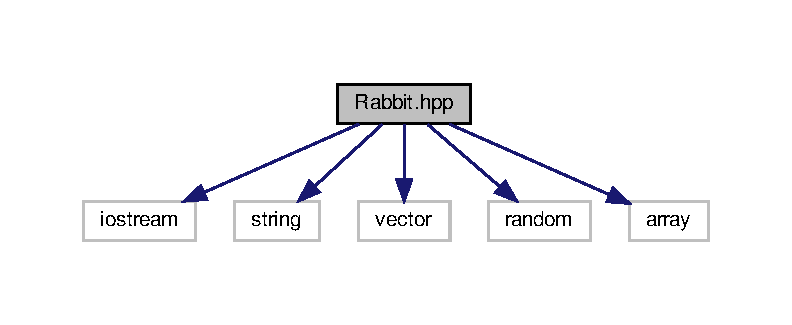
\includegraphics[width=350pt]{Rabbit_8hpp__incl}
\end{center}
\end{figure}
Ce graphe montre quels fichiers incluent directement ou indirectement ce fichier \+:
\nopagebreak
\begin{figure}[H]
\begin{center}
\leavevmode
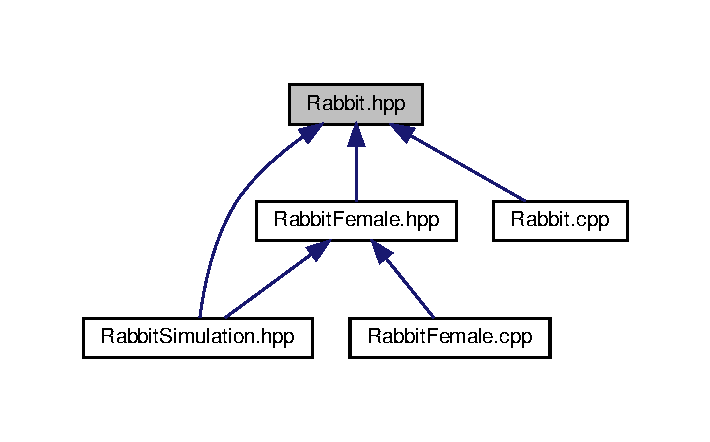
\includegraphics[width=341pt]{Rabbit_8hpp__dep__incl}
\end{center}
\end{figure}
\subsection*{Classes}
\begin{DoxyCompactItemize}
\item 
class \hyperlink{classRabbit}{Rabbit}
\end{DoxyCompactItemize}


\subsection{Description détaillée}
Classe déclarant le comportement d\textquotesingle{}un beau et fort lapin. Contient également l\textquotesingle{}ensembles des distributions nécessaires à la simulation. 

\begin{DoxyAuthor}{Auteur}
Jérémy Z\+A\+N\+G\+LA (\href{mailto:zangla.jeremy@gmail.com}{\tt zangla.\+jeremy@gmail.\+com}) 
\end{DoxyAuthor}
\begin{DoxyVersion}{Version}
1 
\end{DoxyVersion}
\begin{DoxyDate}{Date}
2019-\/11-\/16
\end{DoxyDate}
\begin{DoxyCopyright}{Copyright}
Copyright (c) 2019 
\end{DoxyCopyright}

\hypertarget{RabbitFemale_8cpp}{}\section{Référence du fichier Rabbit\+Female.\+cpp}
\label{RabbitFemale_8cpp}\index{Rabbit\+Female.\+cpp@{Rabbit\+Female.\+cpp}}


Classe décrivant le comportement d\textquotesingle{}une gentille et belle lapine.  


{\ttfamily \#include \char`\"{}Rabbit\+Female.\+hpp\char`\"{}}\newline
Graphe des dépendances par inclusion de Rabbit\+Female.\+cpp\+:\nopagebreak
\begin{figure}[H]
\begin{center}
\leavevmode
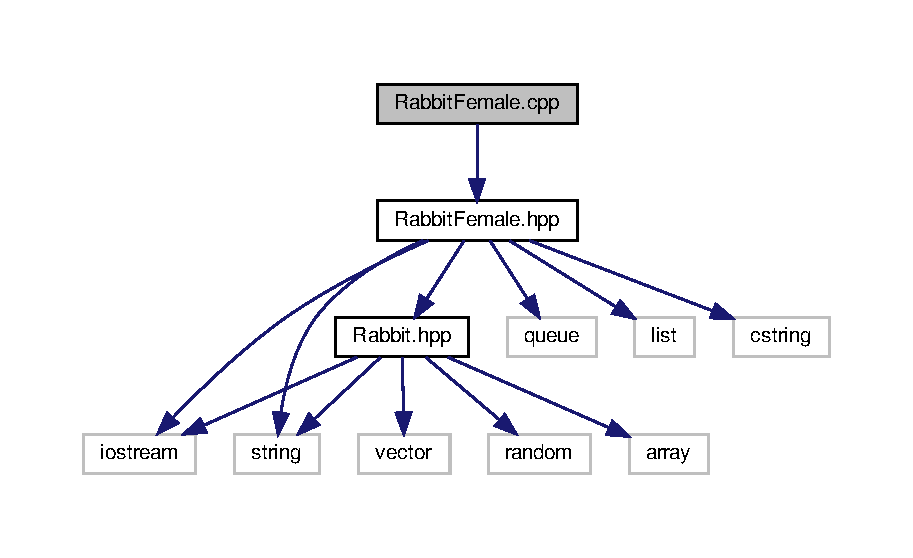
\includegraphics[width=350pt]{RabbitFemale_8cpp__incl}
\end{center}
\end{figure}


\subsection{Description détaillée}
Classe décrivant le comportement d\textquotesingle{}une gentille et belle lapine. 

\begin{DoxyAuthor}{Auteur}
Jérémy Z\+A\+N\+G\+LA (\href{mailto:zangla.jeremy@gmail.com}{\tt zangla.\+jeremy@gmail.\+com}) 
\end{DoxyAuthor}
\begin{DoxyVersion}{Version}
1 
\end{DoxyVersion}
\begin{DoxyDate}{Date}
2019-\/11-\/16
\end{DoxyDate}
\begin{DoxyCopyright}{Copyright}
Copyright (c) 2019 
\end{DoxyCopyright}

\hypertarget{RabbitFemale_8hpp}{}\section{Référence du fichier Rabbit\+Female.\+hpp}
\label{RabbitFemale_8hpp}\index{Rabbit\+Female.\+hpp@{Rabbit\+Female.\+hpp}}


Classe déclarant le comportement d\textquotesingle{}un lapin mâme. Contient également l\textquotesingle{}ensembles des distributions nécessaires à la simulation.  


{\ttfamily \#include $<$iostream$>$}\newline
{\ttfamily \#include $<$string$>$}\newline
{\ttfamily \#include $<$queue$>$}\newline
{\ttfamily \#include $<$list$>$}\newline
{\ttfamily \#include $<$cstring$>$}\newline
{\ttfamily \#include \char`\"{}Rabbit.\+hpp\char`\"{}}\newline
Graphe des dépendances par inclusion de Rabbit\+Female.\+hpp\+:\nopagebreak
\begin{figure}[H]
\begin{center}
\leavevmode
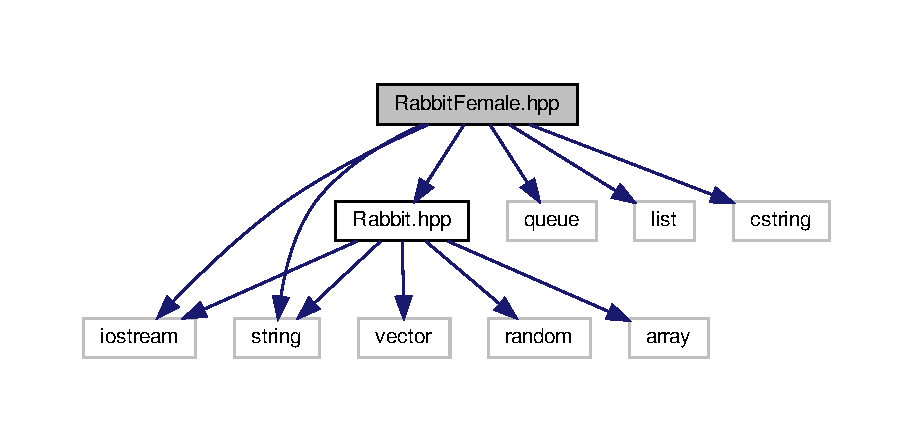
\includegraphics[width=350pt]{RabbitFemale_8hpp__incl}
\end{center}
\end{figure}
Ce graphe montre quels fichiers incluent directement ou indirectement ce fichier \+:
\nopagebreak
\begin{figure}[H]
\begin{center}
\leavevmode
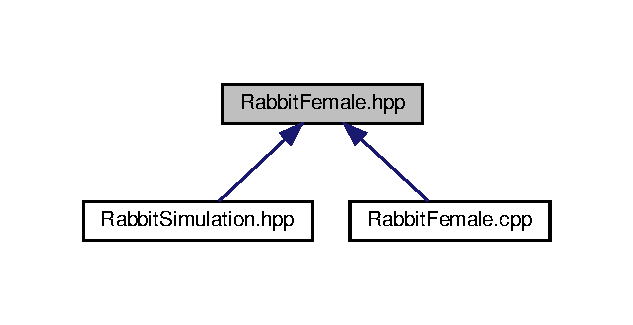
\includegraphics[width=304pt]{RabbitFemale_8hpp__dep__incl}
\end{center}
\end{figure}
\subsection*{Classes}
\begin{DoxyCompactItemize}
\item 
class \hyperlink{classRabbitFemale}{Rabbit\+Female}
\end{DoxyCompactItemize}


\subsection{Description détaillée}
Classe déclarant le comportement d\textquotesingle{}un lapin mâme. Contient également l\textquotesingle{}ensembles des distributions nécessaires à la simulation. 

\begin{DoxyAuthor}{Auteur}
Jérémy Z\+A\+N\+G\+LA (\href{mailto:zangla.jeremy@gmail.com}{\tt zangla.\+jeremy@gmail.\+com}) 
\end{DoxyAuthor}
\begin{DoxyVersion}{Version}
1 
\end{DoxyVersion}
\begin{DoxyDate}{Date}
2019-\/11-\/16
\end{DoxyDate}
\begin{DoxyCopyright}{Copyright}
Copyright (c) 2019 
\end{DoxyCopyright}

\hypertarget{RabbitSimulation_8hpp}{}\section{Référence du fichier Rabbit\+Simulation.\+hpp}
\label{RabbitSimulation_8hpp}\index{Rabbit\+Simulation.\+hpp@{Rabbit\+Simulation.\+hpp}}


Classe déclarant le comportement d\textquotesingle{}une simulation de population de lapin.  


{\ttfamily \#include $<$iostream$>$}\newline
{\ttfamily \#include $<$sstream$>$}\newline
{\ttfamily \#include $<$fstream$>$}\newline
{\ttfamily \#include $<$filesystem$>$}\newline
{\ttfamily \#include $<$string$>$}\newline
{\ttfamily \#include $<$list$>$}\newline
{\ttfamily \#include \char`\"{}Rabbit.\+hpp\char`\"{}}\newline
{\ttfamily \#include \char`\"{}Rabbit\+Female.\+hpp\char`\"{}}\newline
Graphe des dépendances par inclusion de Rabbit\+Simulation.\+hpp\+:
\nopagebreak
\begin{figure}[H]
\begin{center}
\leavevmode
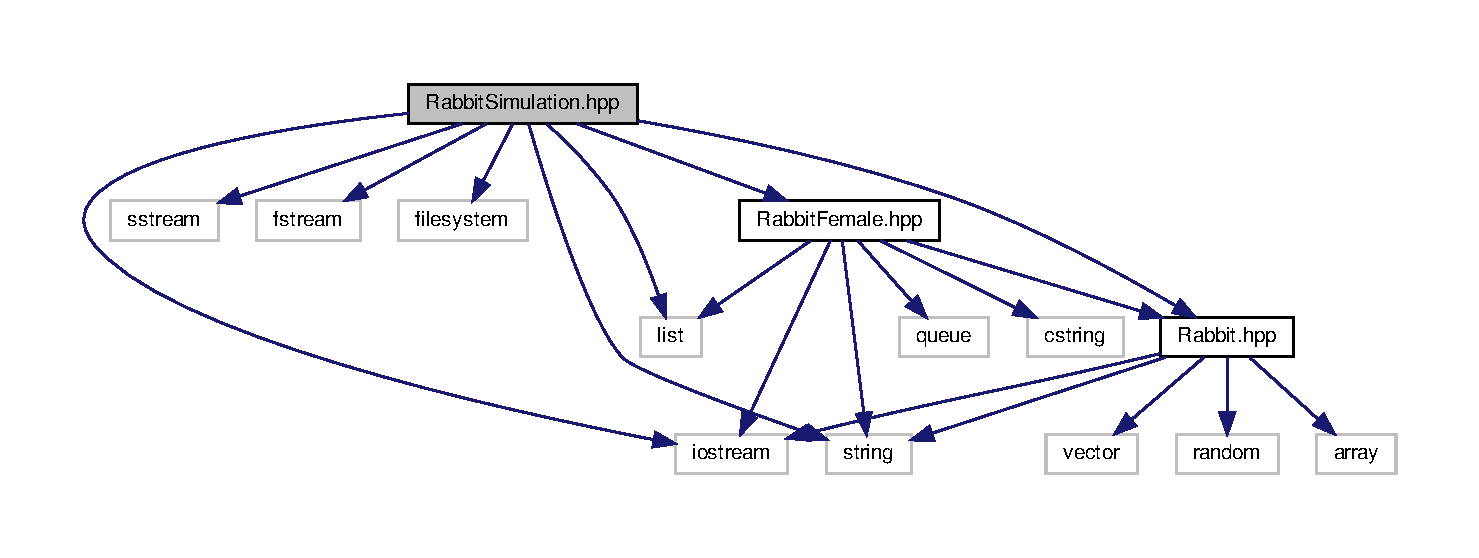
\includegraphics[width=350pt]{RabbitSimulation_8hpp__incl}
\end{center}
\end{figure}
\subsection*{Classes}
\begin{DoxyCompactItemize}
\item 
class \hyperlink{classRabbitSimulation}{Rabbit\+Simulation}
\end{DoxyCompactItemize}


\subsection{Description détaillée}
Classe déclarant le comportement d\textquotesingle{}une simulation de population de lapin. 

\begin{DoxyAuthor}{Auteur}
Jérémy Z\+A\+N\+G\+LA (\href{mailto:zangla.jeremy@gmail.com}{\tt zangla.\+jeremy@gmail.\+com}) 
\end{DoxyAuthor}
\begin{DoxyVersion}{Version}
0.\+1 
\end{DoxyVersion}
\begin{DoxyDate}{Date}
2019-\/11-\/16
\end{DoxyDate}
\begin{DoxyCopyright}{Copyright}
Copyright (c) 2019 
\end{DoxyCopyright}

%--- End generated contents ---

% Index
\backmatter
\newpage
\phantomsection
\clearemptydoublepage
\addcontentsline{toc}{chapter}{Index}
\printindex

\end{document}
